\documentclass[addpoints]{exam}
\usepackage{amsmath,amsthm,amssymb,url}

\usepackage{algorithm}
\usepackage{algorithmic}
\usepackage{graphicx}
\usepackage{float}
\usepackage[pdftex]{hyperref}


\newtheorem{lemma}{Lemma}[section]
\newcommand{\var}{\text{Var}}
\title{CS 6150: HW3}
\date{Due Date: }
\begin{document}
\maketitle
\begin{center}
\fbox{\fbox{\parbox{5.5in}{\centering
This assignment has \numquestions\ questions, for a total of \numpoints\
points.
Unless otherwise specified, complete and reasoned arguments will be expected for all answers. }}}
\end{center}

\qformat{Question \thequestion: \thequestiontitle\dotfill \textbf{[\totalpoints]}}
\pointname{}
\bonuspointname{}
\pointformat{[\bfseries\thepoints]}

\printanswers

\begin{center}
  \gradetable
\end{center}
\newpage



\begin{questions}

\titledquestion{Minimum-cost Tree}

In this problem, the input consists of a complete graph $G=(V,E)$ with distances between all pairs of vertices, and a set $V'\subseteq V$.
Suppose the distances in the input is a metric, and the weight of an edge connecting two vertices in $G$ is defined as the distance between these two vertices.
\begin{parts}



  \part[20] Design  a ratio-2 approximation algorithm to find a minimum-cost tree that includes $V'$. The cost of a tree is the sum of all weights
  of its edges. This tree may or may not include vertices in $V-V'$. Show the approximation ratio of your algorithm is 2. (Hint: Recall the approximation algorithm for the TSP.)
\begin{solution}
In order to design a ratio-2 approximation algorithm to find a minimum-cost tree that includes $V'$, we define the following steps:
\begin{itemize}
\item[a.] Find the minimum spanning tree for the graph $G$.
\item[b.] Double every edge in the minimum spanning tree.
\item[c.] Find an Euler tour.
\item[d.] Short circuit(Remove vertices visited before from the tour).
\end{itemize}
Let $G={V,E}$, where $V=\{A,B,C,D,E\}$ and $E$ is a set of all the edges connecting all vertices in $V$ to each other. \\

Let's take a set $V' \subseteq V$ defined by $\{A,B,C\}$ and $E'$ is a set of all the edges connecting all vertices in $V'$ to each other. As $G$ is a complete graph, hence $G'=\{V',E'\}$ is also a complete graph.\\

Using the steps defined above we find a minimum spanning tree of $G'$ whose cost is minimum of all spanning tree's possible for $G'$. Now lets double the edges of the minimum spanning tree found. Hence taking any vertex in $V'$ as the starting point we find an Euler tour. This results in every path of the minimum spanning tree with doubled edges traveled exactly once which is defined by $C$. We know by observation that $C \leq 2.MST$. Now we perform short circuit of the Euler tour. We know by triangle inequality that the length of an edge connecting $\{u,v\}$ is lesser than or equal to the sum of the remaining $2$ edges. Hence we now that short circuiting is successful as it will always give us a path of smaller distance defined by $C'$. This means that $C'\leq C = 2.MST$. \\

When we find a minimum spanning tree we know that its cost is minimum and an optimal tour of the paths in MST might or might not be equal to the minimum cost.  Hence we can say that $OPT \geq MST$.

Using the inequalities:
\[OPT \geq MST\]\[C'\leq C = 2.MST\]
we get,
\[OPT \geq MST \geq C'/2\]
\[OPT \geq C'/2\]
\[2.OPT \geq C'\]
\[\frac{C'}{OPT} \leq 2\]

Now if we were to add a vertex from $V-V'$ to $V'$ and perform the same steps we will still get the same answer. Hence for any set $V' \subseteq V$, the approximation ratio of our algorithm is 2.\\

\emph{Collaboration with Shweta, Sunny and Yogesh}
\end{solution}

\end{parts}




\titledquestion{Max-SAT Problem}

Suppose you are given a set of clauses, and each clause is the the disjunction of several literals. Your goal is to find an assignment that satisfies as many of these clauses as possible.

\begin{parts}

  \part[8] Here is a simple algorithm:

\begin{algorithm} % enter the algorithm environment
\begin{algorithmic}[1] % enter the algorithmic environment
\FOR { each variable}
\STATE {set its value to either 0 or 1 by flipping a coin}
\ENDFOR
\end{algorithmic}
\end{algorithm}
Suppose the input has $m$ clauses, of which the $j$th has $k_j$ literals, show that the expected number of clauses satisfied by the above algorithm is no less than $\frac{m}{2}$. In other words, this is a $2$-approximation in expectation.
\begin{solution}

The value of each variable or literal is set to 0 or 1 by flipping a coin, therefore each literal has probability of $1/2$. If a clause has $k_j$ literal a clause will not be satisfied i.e clause is false, when all literals in the clause are set to 0. Therefore probability of clause being false is $1/2^{k_j}$ because each variable or literal is independent of each other. Hence the probability of a clause being true is $(1-(1/2)^{k_j})$.\\

Expected number of satisfied clauses are given by $\sum_{j=1}^{m} (1-(1/2)^{k_j})$. As any clause has to have atleast 1 literal, hence $k_j >= 1$. Thereore expected number of clauses satisfied by the above algorithm is no less than $m/2$.\\

\emph{Collaboration with Shweta, Sunny and Yogesh}
\end{solution}

\part[12] Improve the above algorithm to make it deterministic.

\begin{solution}
Instead of flipping the coin we will select the value of the variable that satisfies the maximum number of clauses.\\

For each variable we will first set the value to 0 and calculate the expected number of clauses satisfied. Then we will set the value to 1 and again calculate the expected number of clauses satisfied. Now based on the value that gave max of the expected number of clauses satisfied we will set the value of the variable to it.\\

Example: We are given the the following set of clauses:
\[\overline{X_1},\  X_1 \lor \overline{X_2},\  X_1 \lor X_2 \lor \overline{X_3},\  \overline{X_1} \lor \overline{X_2} \lor \overline{X_3},\  X_1 \lor X_2 \lor X_3\]
where each clause has a weight of 1.  We're expected to get a weight of:
\[\frac{1}{2}+\frac{3}{4}+\frac{7}{8}+\frac{7}{8}+\frac{7}{8} = 3\frac{7}{8}\]
If we set $X_1$ = False we get an expectation of:
\[1+\frac{1}{2}+\frac{3}{4}+1+\frac{3}{4} = 4\] 
If we set $X_1$ = True we get an expectation of:
\[0 + 1 + 1 +\frac{3}{4}+1 = 3\frac{3}{4}\]

Therefore, we'll set $X_1$ = False.  Let's continue to setting the second variable.  If we set $X_2$ = False we get an expectation of:
\[1 + 1 +\frac{1}{2}+1+\frac{1}{2} = 4\]
If we set $X_2$ = True we get an expectation of:
\[1 + 0 + 1 + 1 + 1 = 4\]
Notice that if we set $X_2$ = True we decide which of the clauses are satisfied deterministically, and we get that the total weight is higher than the initial expectation.\\

\emph{$http://www.cs.tau.ac.il/\mathtt{\sim}azar/Methods-Class6.pdf$}

\end{solution}
\end{parts}


\titledquestion{Containers and Truck}
 Suppose a ship arrives, with $n$ containers of weight $w_1,w_2,\cdots,w_n$. Standing on the dock is a set of trucks, each of which can hold $K$
 unites of weight. (You can assume that $K$ and each $w_i$ is an integer.) You can stack multiple containers in each truck, subject to the weight
 restriction of $K$; the goal is to minimize the number of trucks that are needed in order to carry all the containers.
 
 A greedy algorithm you might use for this is the following. Start with an empty truck, and begin piling containers $1, 2, 3, \ldots $ into it until you get to a container that would overflow the weight limit. Now declare this truck "loaded" and send it off; then continue the progress with a fresh truck. This algorithm, by considering trucks one at a time, may not achieve the most efficient way to pack the full set of containers into an available collection of trucks.
 

\begin{parts}
  \part[5] Give an example of a set of weights, and a value of $K$, where this algorithm does not use the minimum possible number of trucks.
  
\begin{solution}

Let's consider $n=5$ and the weights of the containers as $ 1,2,3,4,5$ and the weight that a truck can hold i.e, $K = 5$(as the trucks should be able to carry more than or equal to the maximum weight).
The minimum no of trucks required by the Greedy algorithm as mentioned are: $3$
as, truck 1 will contain containers of weight $1,2$ i.e,$3$, Later when container with weight $3$ arrives it can not be placed on truck 1, so truck 2 will accommodate $3$, truck $3$ will contain the container $4$ and truck $4$ will accomodate container $5$.
We can see that none of the truck's load is optimized.The optimal solution would be to first let all the containers arrive and then optimally place containers on the trucks, so that the load of a truck can be optimized to maximum.

Total weight of all the containers in the given scenario is $15$.So according to the $K=5$, the no of trucks should be $3$.
Solution would be: Truck 1 will contain containers with weight $1,4$, truck 2 will be having $2,3$ weight containers and truck 3 will be having $5$.

Here, the number of trucks required to carry all the containers is less than the number of trucks required to carry containers using the Greedy Algorithm.\\

\emph{Collaboration with Shweta, Sunny and Yogesh}
\end{solution}

  \part[15] Show, however, that the number of trucks used by this algorithm is within a factor of  $2$ of the minimum possible number, for any set of weights and any value $K$.

\begin{solution}
$T$ is the total number of trucks and $T^*$ be the optimal solution which will be greater than equal to the total weight of containers divided by the capacity of each truck $\left(T^* \geq \frac{1}{K}\sum_i^n w_i\right)$. Let $S_i$ denote the set of weights that truck $i$ loads. By analyzing the greedy algorithm we can conclude that two sequential trucks loads $S_i$ and $S_{i-1}$ respectively and that the following must hold for any $i$:
$$\mid S_i \mid + \mid S_{i-1} \mid = \sum_{w_j \in S_i}w_j + \sum_{ w_k \in S_{ i - 1}} w_k > K $$
which means that a truck $i$ loads $l_i > K/2$ on average. Furthermore, we have that
\[\sum_{k=1}^n w_k = \sum_{i=1}^T \sum_{w_j \in S_i} w_j = \sum_{i=1}^T \mid S_i \mid\]

If we have an even number of trucks $T = 2T'$ then
\[\sum_{i=1}^T \mid S_i \mid = \sum_{i=1}^{T'}\left( \mid S_{2i} \mid+ \mid S_{2i-1} \mid \right) > \sum_{k=1}^{T'}K = \frac{1}{2}TK\]
and for an odd number of trucks $T = 2T'+ 1$ then
\[\sum_{i=1}^T \mid S_i \mid = \mid S_T \mid + \sum_{i=1}^{T'} \left( \mid S_{2i} \mid + \mid S_{2i-1} \mid \right) > \sum_{k=1}^{T'}K = \frac{1}{2}(T-1)K\]

From above two inequalities we can infer that for any solution T
\[\sum_{i=1}^T \mid S_i \mid > \frac{1}{2} (T-1)K \]

since, clearly, $\frac{1}{2} \left( T-1 \right)K < \frac{1}{2}TK$. Using second inequality
\[\frac{1}{2} \left(T-1 \right)K < \sum_{k=1}^n w_k \Rightarrow T \leq 2 \frac{1}{K}\sum_{i=1}^n w_i\]
but $T^* \geq \frac{1}{K} \sum_i ^ n w_i$ then $T \leq 2T^*$.\\

\emph{http://web.engr.illinois.edu/~jeffe/teaching/algorithms/notes/31-approx.pdf}\\
\emph{http://homepage.cs.uiowa.edu/~hzhang/c231/ch11.pdf}\\
\emph{http://per.lindstrand.org/docs/adv\_algo\_1.pdf}

\end{solution}
  
  
\end{parts}




\titledquestion{Grid Graph}

   Suppose you are given an $n\times n$ grid graph $G$ as in the following figure.

\begin{figure}[H]
  \centering
  % Requires \usepackage{graphicx}
  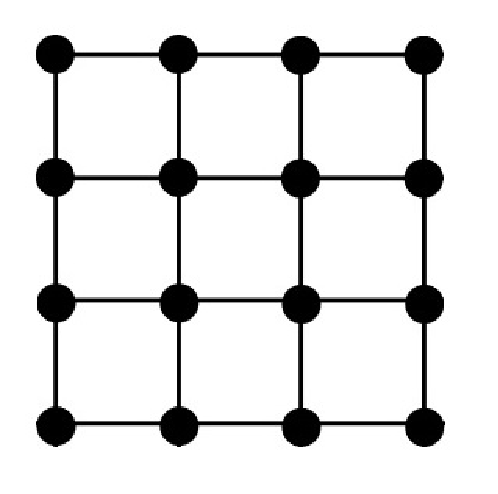
\includegraphics[width=0.3\textwidth]{fig1.pdf}\\
  \caption{A grid graph.}
\end{figure}

Associated with each node $v$ is a weight $w(v)$, which is a nonnegative integer. You may assume that the weights of all nodes are distinct.
Your goal is to choose an independent set $S$ of nodes of the grids, so that the sum of the weights of the nodes on $S$ is as large as possible.
(The sum of the weights of the nodes in $S$ will be called its total weight.)


Consider the following greedy algorithm for this problem.
\begin{algorithm*} % enter the algorithm environment
\caption{The "heaviest-first" greedy algorithm:} % give the algorithm a caption
\begin{algorithmic} % enter the algorithmic environment
\STATE Start with $S$ equal to the empty set
\WHILE {some node remains in $G$}
\STATE Pick a node $v_i$ of maximum weight
\STATE Add $v_i$ to $S$
\STATE Delete $v_i$ and its neighbors from $G$
\ENDWHILE
\RETURN $S$
\end{algorithmic}
\end{algorithm*}



  \begin{parts}
    \part[7] Let $S$ be the independent set returned by the "heaviest-first" greedy
    algorithm, and let $T$ be any other independent set in $G$. Show that, for each node $v\in T$, either $v\in S$, or there is a node $v'\in S$ so that $w(v)\leq w(v')$ and $(v,v')$ is an edge of $G$.
\begin{solution}
Proof by contradiction: Suppose there exists $v\in T$ such that $v\notin S$ and $v$ has no neighbor $v' \in S$ such that $w(v) \le w(v')$. Then we know that at least one of $v$'s neighbors must be in $S$, since at least one of $v$ and its adjacent nodes must be in $S$. Suppose $v'\in S$ is $v$'s neighbor, then at the time $v'$ is added to $S$, $v$ must still remains, because $v$ has no neighbor with a greater weight and $v\notin S$, but according to the "heaviest-first" algorithm, $v'$ cannot be added to $S$, because it is not the heaviest weight node ($w(v)>w(v')$). This is a contradiction. So for each node $v \in T$, either $v \in S$, or there is a node $v'\in S$ so that $w(v) \le w(v')$ and $(v, v')$ is an edge of $G$.

\end{solution}

\part[13] Show that the "heaviest-first" greedy algorithm returns an independent set of total
    weight at least $\frac{1}{4}$ times the maximum total weight of any independent set in the grid graph $G$.
\begin{solution}

We know that any node $v$ in $G$ has at most 4 neighbors. So for any independent set $T$, up to 4 nodes from $T-S$ can share one node from $S-T$ as their common neighbor. As $T$ is any independent set we can say that:\\
\[\sum_{v\in T}w(v) =\sum_{v\in T}w(v)\]
As atmost 4 nodes in $T-S$ may be neighbours of a node in $S-T$ and weight of each node in $T-S$ will be less than equal to the weight of node in $S-T$, hence:\\
\[\sum_{v\in T}w(v) \le 4\sum_{v'\in S}w(v')\]\[\sum_{v'\in S}w(v') \ge \frac{1}{4}\sum_{v\in T}w(v)\]

Therefore the ``heaviest-first'' greedy algorithm returns an independent set of total weight at least 1/4 times the maximum total weight of any independent set in the grid graph $G$.\\

\emph{http://spotidoc.com/doc/762193/solutions}
\end{solution}

\end{parts}

\titledquestion{Graph Coloring}[20]

Solve Question 8, parts (a), (b) \textbf{ONLY} from
\url{http://web.engr.illinois.edu/~jeffe/teaching/algorithms/notes/31-approx.pdf}. Each
part is worth 10 points. 
\begin{solution}
\begin{parts}
\part{} Lets take a bipartite graph $G$ and take a spanning tree $T$ of $G$. We know that bipartite graphs have two sets of vertices which are connected by edges but the vertices in the same set are not connected to each other directly. By property of trees we know that any tree is a bipartite graph.

Now we will color all the vertices in the   spanning tree of a bipartite graph with  2 colors. We also know that a tree is always 2-colorable which means that no neighbor of a vertex has the same color. For every edge $\{u,v\}$ in $G - T$, we will add the edge to $T$. As the color of vertices $u$ and $v$ are different we will never enter any of the conditions in the loop.

Therefore this algorithm colors any bipartite graph with just two colors.

\part{}
We will prove the statement $P(n)$ by induction:\\
Statement: Any graph $G$ with  $n$ vertices and a maximum degree of $\Delta(G)$ is colorable with atmost $\Delta(G)+1$ colors.\\

Basis: For $G$ with $n=1$ vertices, $\Delta(G)$ is 0. If we apply the algorithm, the spanning tree will be the vertex itself. The vertex will be colored with 1 color. as there are no edges hence the loop will not run. Therefor the graph $G$ with maximum degree of $\Delta(G)$ is colorable with atmost $\Delta(G)+1$ colors.\\

Inductive Step:
\begin{itemize}
\item[1.] Lets consider that $P(n)$ is true for $n$ vertices with maximum degree $\Delta(G) = k$, hence $G$ is colored using atmost $\Delta(G)+1 = k+1$ colors.
\item[2.] Now we will prove that $P(n)$ is true for $n+1$ vertices with maximum degree $k$.
\item[3.] Lets remove a vertex $v$ from the $n+1$ vertices(and all its edges), leaving a graph with $n$ vertices and maximum degree $k$. We know that a graph with $n$ vertices with maximum degree $k$ is $k+1$ colorable.
\item[4.] Now add the vertex $v$ back to the graph. We can assign $v$ a color from the set of $k+1$ colors, as $v$ can have atmost $k$ neighbours and atleast one of the $k+1$ colors will be available.
\item[5.] Therefore graph $G$ is $k+1$-colorable.

\end{itemize}
Hence $P(n)$ is true as proved above by induction.
\end{parts}
\end{solution}

\textbf{BONUS:} for 10 extra points, solve Question 8(c). Note that you will
solve this by constructing an example graph of size $n$ and showing that you
need $\omega(1)$ colors. 
\begin{solution}
Let's take a graph $G$ with $n = 4$ vertices and $G$ is a complete graph. We will also consider a fixed number of colors, say 2 colors. 

Now lets run the algorithm on the graph $G$. We first get a spanning tree $T$ from $G$ which is 2-colorable as per the property of a tree. Now from every edge $\{u,v\}$ in $G-T$ we add edge to $T$. We will get an edge where both the vertices have the same color. Similarly we will also have the situation where the neighbors have the fixed colors used as well as a vertex with same color. Now as per the algorithm we will have to assign a new color apart from the fixed number of colors. 

Hence, the TREECOLOR algorithm is not  a constant approximation algorithm.

Alternatively, the same was also proved in \emph{$5(b)$} that my approximation algorithm is dependent on $\Delta(G)$ which is the maximum degree. This is never constant for all graphs $G$ as they all can have  different $\Delta(G)$.
\end{solution}
\end{questions}
\end{document}
